% efficiency_index_full.tex -- self-contained standalone figure
\documentclass[tikz]{standalone}
\usepackage{pgfplots}
\pgfplotsset{compat=1.18}
\usepgfplotslibrary{groupplots}
\usepackage{siunitx}

\begin{document}
\begin{figure}[htbp]
\centering
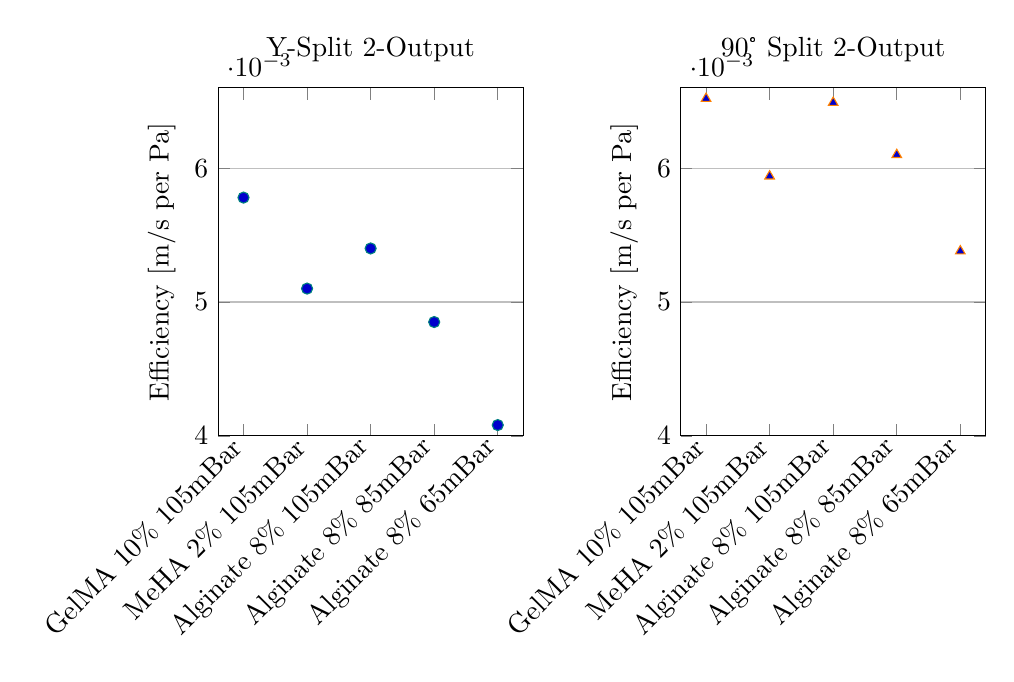
\begin{tikzpicture}
\begin{groupplot}[
  group style={group size=2 by 1, horizontal sep=2cm},
  width=0.45\textwidth, height=6cm,
  ymajorgrids=true,
  xtick=data,
  xticklabel style={rotate=45, anchor=east},
  xlabel={}, ylabel={Efficiency [m/s per Pa]},
  ymin=0.004, ymax=0.0066
]

% LEFT PLOT — Y-Split
\nextgroupplot[
  title={Y-Split 2-Output},
  symbolic x coords={
    GelMA 10\% 105mBar,
    MeHA 2\% 105mBar,
    Alginate 8\% 105mBar,
    Alginate 8\% 85mBar,
    Alginate 8\% 65mBar
  }
]
\addplot+[only marks, mark=*, color=teal] coordinates {
  (GelMA 10\% 105mBar, 0.00578)
  (MeHA 2\% 105mBar, 0.00510)
  (Alginate 8\% 105mBar, 0.00540)
  (Alginate 8\% 85mBar, 0.00485)
  (Alginate 8\% 65mBar, 0.00408)
};

% RIGHT PLOT — 90° Split
\nextgroupplot[
  title={90° Split 2-Output},
  symbolic x coords={
    GelMA 10\% 105mBar,
    MeHA 2\% 105mBar,
    Alginate 8\% 105mBar,
    Alginate 8\% 85mBar,
    Alginate 8\% 65mBar
  }
]
\addplot+[only marks, mark=triangle*, color=orange] coordinates {
  (GelMA 10\% 105mBar, 0.00652)
  (MeHA 2\% 105mBar, 0.00594)
  (Alginate 8\% 105mBar, 0.00649)
  (Alginate 8\% 85mBar, 0.00610)
  (Alginate 8\% 65mBar, 0.00538)
};

\end{groupplot}
\end{tikzpicture}
\caption{Efficiency index (velocity divided by wall shear stress) for 2-outlet Y-split and 90-degree designs across all bioinks and pressure conditions. Higher values represent greater extrusion efficiency.}
\label{fig:efficiency_index}
\end{figure}
\end{document}
